\chapter{Improving the Output} % Main chapter title

\label{Chapter5} % Change X to a consecutive number; for referencing this chapter elsewhere, use \ref{ChapterX}

\lstset{language={},
showstringspaces=false,
numbers=none,
}

%----------------------------------------------------------------------------------------
%	SECTION 1
%----------------------------------------------------------------------------------------
\todo{Add intro. Why we're doing this, etc.}

\section{Creating a Simple Log}

The first step in improving the output of the test framework is improving the log output.
To do this, it was decided that a simple log file should be created for several reasons.
The log files produced by the test framework have a considerable amount of detail contained within them, however this comes at the cost of being incredibly large — even a relatively simple test such as DualType (produced in the previous section) can create log files of 4,000+ lines.
More than that, the log files produced are very difficult to follow, as they are ordered by log file, then chronologically.
Meaning that following a chain of events between multiple nodes becomes a process of consistently switching between sections of log file.
Further, the log files produced by the test framework have several issues: the formatting is inconsistent, timestamps are in different formats, a lack of information around network topology, and some log messages are either too verbose or do not contain enough information.

To fix this, the simple log will require six main features.
\begin{itemize}
    \item Consistent formatting
    \item Chronological ordering by timestamp
    \item Reduce amount of information to only useful info
    \item Machine \emph{and} human-readable layout information
    \item Log traceability to original log file
    \item Support all pre-existing topology tests
\end{itemize}


Several options exist for creating a simple log.
The first is to modify the pre-existing codebase of LBARD, Servald, Fakeradio, and the test framework, and modify their logging to meet the above requirements.
This is not considered to be a useful use of this thesis, as this would require changing large parts of the codebase for these programs for a relatively mild improvement, as well as modifying the code of tested and running devices.

The next is to modify the test framework to process and modify the log lines while the tests are run before piping them to the log file.
While this does solve the issue of the previous proposed solution this would add a large amount of bloat to the test framework that is not required in the vast majority of the tests, and may actually prove to be either impossible or vastly difficult using the Shell scripts of the test framework.
Further, this will increase the run-time for tests unnecessarily.

The final option is to write a program that after a test is run and the log file produced, processes the log file and filters and simplifies it, and outputs a separate, simpler log file. 
This is the method that will be undertaken in this thesis. 
The program will be written in C as it needs to be fast, portable, and use minimal external dependencies, as well as it is the language that the majority of the Serval codebase is written in — allowing for future developers to easily maintain and improve the code.

As shown in \figurename{ \ref{fig:chapter5SimpleFlowchart}}, the program follows a simple process.
For each line in the log file, two steps are followed.
First, the line is filtered to determine if it should appear in the simple log file. 
Then, for each line that passes through the filter, apply some transformations to it if necessary so it is in a more useful format.
Different transformations may be used for different types of lines in the log file.


\begin{figure}
    \begin{centering}
        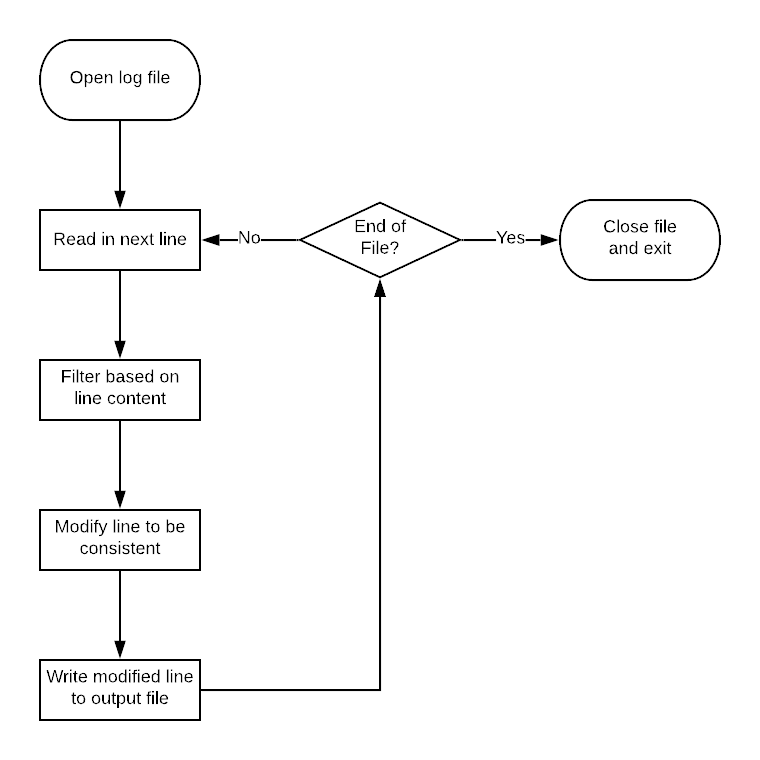
\includegraphics[width=10cm,height=20cm,keepaspectratio]{Figures/Chapter5-SimpleLogFlowchart.png}
        \caption{Flowchart of creating the simple log}
        \label{fig:chapter5SimpleFlowchart}
    \end{centering}
\end{figure}

\subsection{Filtering Lines}\label{filteringLines}
\begin{itemize}
    \item Why they are chosen
\end{itemize}

To ensure that the simple log contains only important lines, the input file needs to be filtered.
Filtering the log file allows for the simple log to contain only lines that are crucial to understanding the operating of the test without overwhelming the person examining the log file.

To determine the minimal information required to understand the tests, the output log files of the tests were analysed.
While analysing the output log files, the following list of important events was created.
\begin{itemize}
    \item \textbf{Setup} Start of a process, LBARD/Fakeradio
    \item \textbf{Setup} Test details
    \item \textbf{Setup} Layout information (WiFi and Fakeradio)
    \item \textbf{Setup} SID information
    \item \textbf{Servald} Sending and receiving packets
    \item \textbf{Servald} Adding manifest
    \item \textbf{LBARD} Neighbour has a bundle
    \item \textbf{LBARD} Send and receive bundles
    \item \textbf{Fakeradio} Any transfer between two nodes
\end{itemize}
\todo{Update this to the latest details}
This list covers all major aspects of a topology test; transfer of bundles, setup and layout information, sending and receiving general packets (including the tree-sync packets), and some internal logic and processing when packets are sent and received.
With only these important events, it should be possible to locate and isolate issues related to transferring bundles and packets. 
From there, these filtered events should allow a tester to more easily utilise the vastly more expansive and detailed original log file produced by the test framework. 

Once the desired events had been determined, these then needed to be filtered within the program.
To achieve this, each line in the file is analysed to determine if it is important by examining what substrings the line contains.
A line is accepted if it matches specified criteria; for instance, a line within the Fakeradio process that contains the substring "neighbour has a bundle" would be considered important. 
These lines are then sent to the relevant function to be formatted appropriately.

\subsection{Output format}

\subsubsection{Formatting lines}
The log files produced by the test framework follow a consistent structure.
The structure always follows the structure of:
\begin{itemize}
    \item the test details, 
    \item the output of the test framework, 
    \item output of Fakeradio, 
    \item output of \emph{each} LBARD process, and finally,
    \item the output of \emph{each} Servald process.
\end{itemize} 

This structure means that filtering each line becomes far simpler, since we only need to track which process (Fakeradio, LBARD, Servald) we are in, and then filter lines within that process that are relevant.
However, the test framework log files have one major issue: the format of lines is not consistent between processes.
For instance, the typical Servald line may look like
\begin{center}
    \begin{lstlisting}[basicstyle=\small, breaklines]
DEBUG:[511710] 18:15:34.372 overlay_mdp.c:859:_overlay_send_frame() {mdprequests} Send frame 68 bytes    
    \end{lstlisting}
\end{center}
while a similar line in LBARD may look like:

\begin{center}
    \begin{lstlisting}[basicstyle=\small, breaklines]
T+25138ms : Sending length of bundle 6A1A3379501553D1* (bundle #0, version 1596098704035, cached_version 1596098704035)
    \end{lstlisting}
\end{center}


As can be clearly seen, there is a huge difference in format between these two lines, and as such these need to be formatted differently.
To achieve this, when a line is filtered as outlined in the previous section, the program returns an integer value representing the type of line that is to be formatted.
With this information, the appropriate function can be called for the line type, so that it can be formatted correctly.

For Servald lines this becomes trivial, simply use the \verb|sscanf| function to extract the important information from the line, format and write this to a variable using the \verb|sprintf| function, and then write this line to the output file. 
However, in the case of LBARD and Fakeradio lines, multiple issues arise due to the formatting of the log files.
The first of these issues is that several lines in LBARD are not timestamped with the time that they occurred, rather they are timestamped with the number of milliseconds since the program started.
This is an issue since this means that the log files can not be easily sorted by timestamp, and also will not be formatted with a consistent format with the other lines.
To fix this, the initial time that an LBARD instance is started as logged by the file will be used as the T=0 point.
After this has occurred, when an event with a 'T+' timestamp is encountered, the number of milliseconds is added to the original timestamp to produce an accurate timestamp for this event.

The other issue with this method is that Fakeradio log lines often are spread over multiple lines.
This means that simply scanning and processing a single line will not produce all the necessary information.
However, when 
\todo{Finish this}

\subsubsection{Output log file}
\todo{Add sorting the output}

Once the log file has been produced it follows a consistent format.
The simple log files format begins with the setup section.
The setup section lists all the essential information for drawing a diagram of the network topology. 
It lists the test details, SIDs of each of the nodes, and all the WiFi connections and Fakeradio rules. 
An example of the setup section can be seen in \figurename{ \ref{fig:chapter5SimpleLogSetup}}.

\begin{figure}
    \begin{centering}
\begin{lstlisting}[frame=single]
#000 ====== BEGIN SETUP ======
#001 Name:     Wifi_RFD900_Chain_Short (topologies)
#002 Result:   PASS
#003 Started:  2020-08-24 13:22:55.044
#004 Finished: 2020-08-24 13:23:32.497
#005 SIDA : F170309E3033B957*
#006 SIDB : 86C9DD08EA6A4C65*
#007 SIDC : FA71E8E919914B52*
#008 SIDD : 41A35E8851578F82*
#009 SIDE : 954B6D94024986A0*
#010 SIDF : B38FB12CB39D006C*
#011 B connected to wifi interface 1
#012 C connected to wifi interface 1
#013 D connected to wifi interface 2
#014 E connected to wifi interface 2
#015 RULE: 'allow between 0,1'
#016 RULE: 'allow between 2,3'
#017 RULE: 'allow between 4,5'
#018 RULE: 'deny all'
#100 ======= END SETUP =======    
\end{lstlisting}
    \caption{Format of simple log setup}
    \label{fig:chapter5SimpleLogSetup}
    \end{centering}
\end{figure}

After the setup section each line in the log file is ordered by chronological order. 
The lines follow a simple and consistent structure.
\begin{center}
    \begin{lstlisting}[basicstyle=\small, breaklines]
[Timestamp] [Process]:[Instance Letter] [Description]
    \end{lstlisting}
\end{center}

This structure can be seen in \figurename{ \ref{fig:chapter5SimpleLogFormat}}.
\begin{figure}
    \begin{centering}
\begin{lstlisting}[basicstyle=\small, breaklines, frame=single]
13:23:18.358 LBARD:A Resending bundle 3580786E* from the start.
13:23:18.358 LBARD:A Sending length of bundle 3580786E* 
13:23:18.370 FAKERADIO A -> B [Bundle end piece ] [218 bytes]
13:23:18.370 FAKERADIO A -> B [Time stamp] [218 bytes]
13:23:18.370 LBARD:A I just sent manifest piece [128,258) for 86c9dd08ea6a*.
13:23:18.388 LBARD:B : Calling message handler for type 'S' @ offset 0x15
13:23:18.388 LBARD:B : Calling message handler for type 'T' @ offset 0x8
13:23:18.388 LBARD:B : Calling message handler for type 'p' @ offset 0x21
13:23:18.388 LBARD:B Decoding message #4 from f170309e3033*, length = 186:
13:23:18.388 LBARD:B We have the entire bundle 3580786E*    
\end{lstlisting}
        \caption{Format of simple log events}
        \label{fig:chapter5SimpleLogFormat}
    \end{centering}
\end{figure}


\section{Drawing Packet Transfer through the network}
To improve the output of the test framework, a network diagram displaying packet transfer is highly useful, allowing testers to better understand the topology they are testing. To produce a useful and informative network diagram, four steps need to be undertaken: determine the major events to be displayed on the diagram, create an ASCII representation of events during a test, generate a network diagram, and finally, create a PDF of the network topology with the traffic displayed.


\subsection{Getting Major and Minor events}
To create our network diagrams, we first need to determine what will be displayed on the diagram.
To do this, two categories of log messages are defined: 
\begin{list}{}{}
    \item Major: When a node sends a message/packet to another
    \item Minor: Some processing on a single node that would not give the full picture of the test if omitted
\end{list}

Major events will be displayed in a diagram showing the network layout, showing the transfer between the two nodes and the message details. 
Minor events however, will be displayed in a list of minor events that occurred before the major event.
There can be multiple minor details per major event, however there is only one major event for each minor event.

There are two options for processing and sorting major and minor events.
The first is to simply process the simple log after it has been made, and check if a line should be considered major or minor. 
The other solution is to classify lines as they are processed in the creation of the simple log.
The second option is quite clearly considerably faster, as in the first option we must re-process a new file and then classify lines within it to be major or minor, however the second option has a major issue in that when lines are classified during the creation of the simple log they are not yet sorted.
This means that if an array of major and minor events is created then these events will \emph{not} be in chronological order.
Unsorted events is a major issue for the creation of diagrams as the created diagrams will quite obviously not be ordered.
This means that for the second option to be considered, a method of sorting and \emph{then} assigning minor events to a major event must be developed.
This is the approach that this thesis took.

Determining major events is relatively simple; major events are a transfer between two nodes.
To effectively save major events, a struct defining major events is created.
This struct contains all the necessary features of a major event. These details are:
\begin{itemize}
    \item Sending Node
    \item Destination Node
    \item Transfer details (type of message, size, etc.)
    \item The time it occurs at
    \item The transfer type (Fakeradio or WiFi)
    \item An array of minor events associated with this major event
\end{itemize}
This occurs at two different points in the log file: when Fakeradio sends a packet to a different node, and when Servald sends a packet.
Fakeradio events are already filtered down to a one line log event for the simple log, so the program simply breaks this line down to get the details of the event, and then appends this to the major events array.
Servald events however are more complicated as the packet transfer takes place over several messages.
To convert this into one event, the program simply saves the details of the packet as each line is processed until the log line stating that the message is sent, at which point all the saved details are added to an event and appended to the major event array.


To add the minor events, when a line for the simple log is being formatted for the simple log, the program simply checks if it meets a handful of criteria.
The minor events that are filtered include:
\begin{itemize}
    \item Add stuff here
    \item to-do
\end{itemize}
\todo{Add the list of filtered things}
\todo{Make all log lines?}
Since the log lines are just a single line, saving these minor events is as simple as appending these lines to the minor event array.


Once the simple log file has been produced, and all major and minor events have been extracted, each minor event needs to be associated with a major event.
When major and minor events are added to their respective arrays, they are done so in the order that the relevant lines appear in the input log file, meaning that these arrays are not chronologically sorted.
To associate a minor event with a major event, the minor event must occur before a major event, but \emph{after} the proceeding major event.
To achieve this, both of the arrays must be sorted.
This is simple to achieve using the C standard function \verb|qsort|.
To use this function, a comparator needs to be implemented: that is to say, a function that is able to compare two objects and return a number indicating which object is bigger.
As major events are stored as a struct with a timestamp field the comparator for this is simple to implement; convert the timestamps to a long, and determine which is larger.
For minor events this is similar; extract the timestamp from the message, convert this timestamp to a long, then determine which is larger.
With these comparators implemented, both the major and minor event arrays can be quickly sorted.
Using the sorted arrays, the program is now able to assign minor events to major events.
The process to do this is simple. Iterate through every major event, and check if the top item in the minor events array occurs before the major event.
If it is, then add it to the major event and move to the next minor event. 
Do this for every minor event until a minor event is reached that is after the major event.
At this point, iterate to the next major event and repeat this process.
This is done until all major events have been processed.
The process for combining major and minor events can be seen in \figurename{ \ref{fig:chapter5CombineMajorMinor}}.

With all the minor events assigned in chronological order to a relevant major event, an ASCII representation of the network traffic throughout the test can be created.

\begin{figure}
    \begin{centering}
        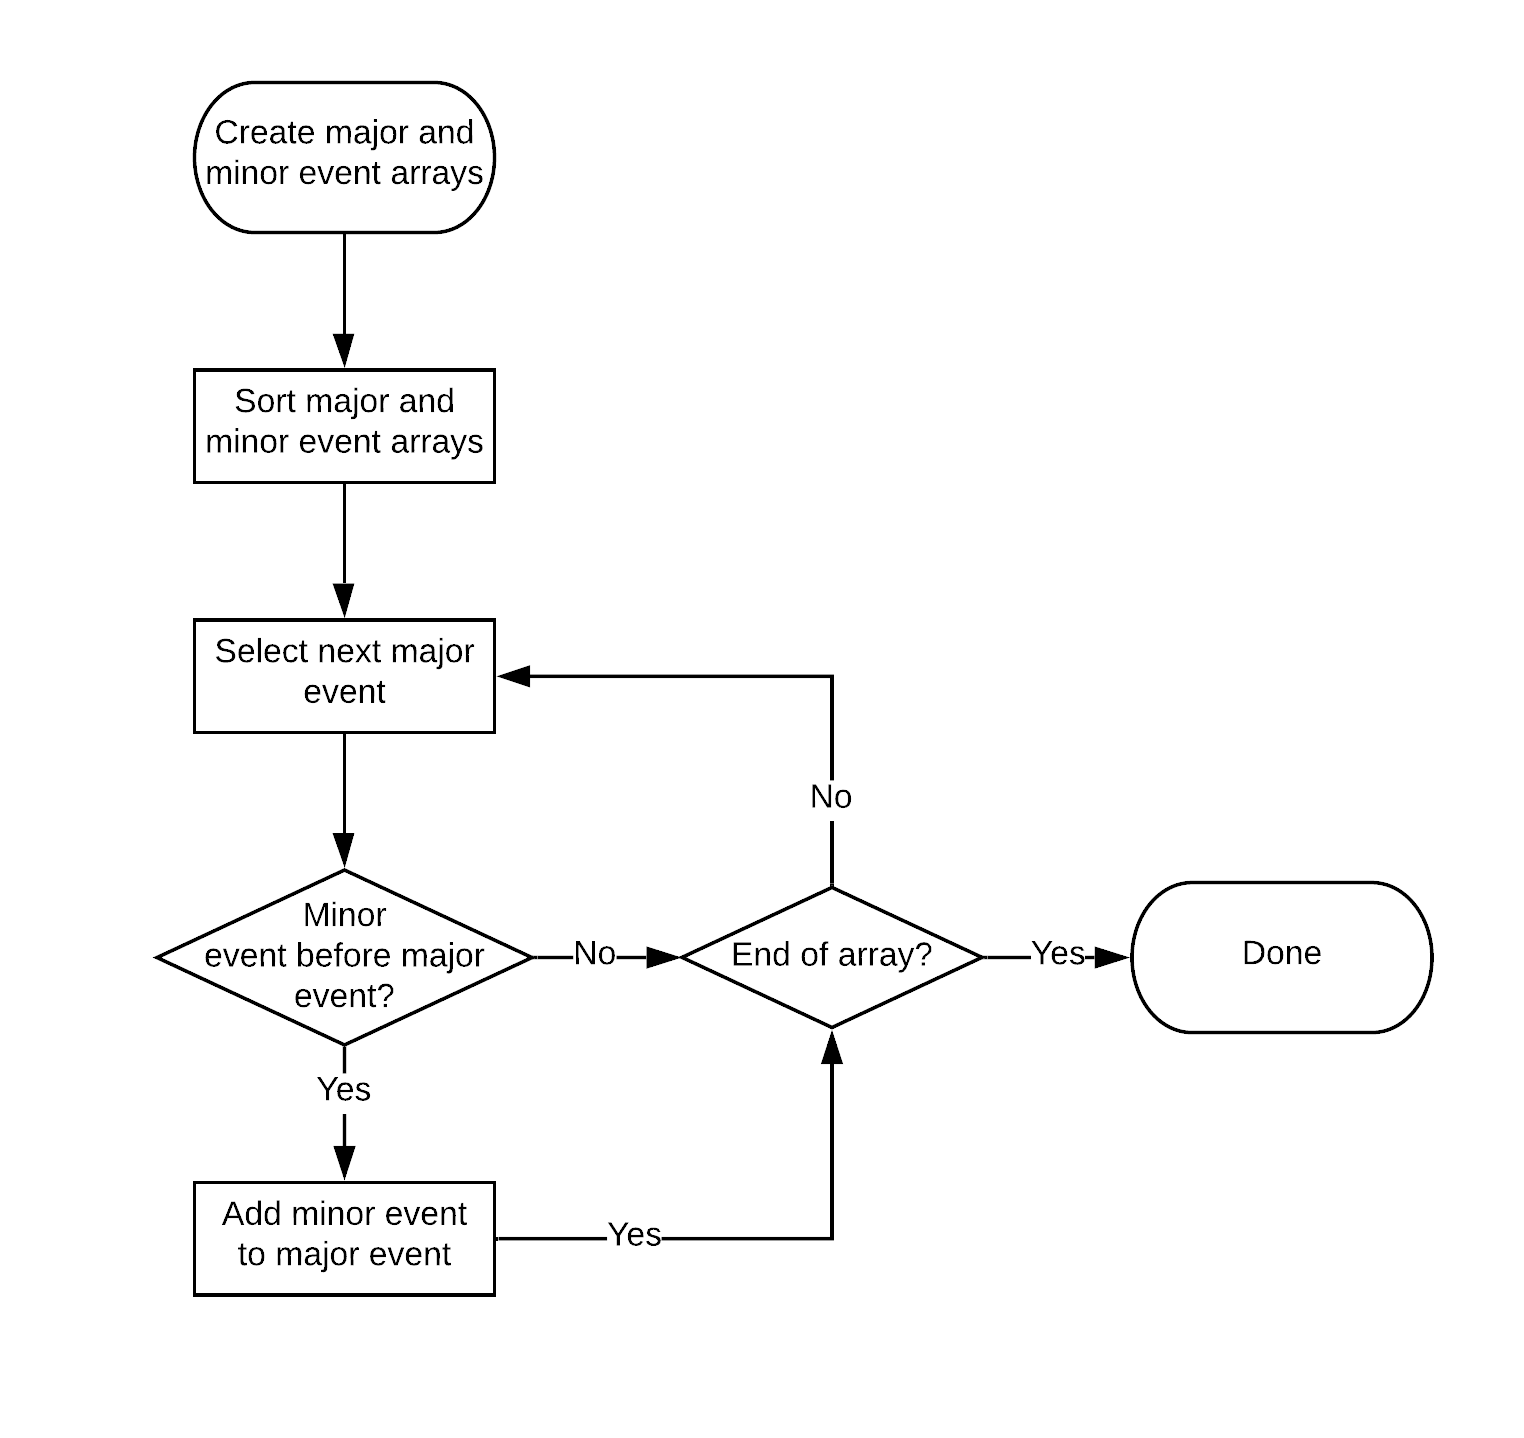
\includegraphics[width=10cm,height=15cm,keepaspectratio]{Figures/Chapter5-CombiningMajorMinor.png}
        \caption{Process of combining Major and Minor events}
        \label{fig:chapter5CombineMajorMinor}
    \end{centering}
\end{figure}

\subsection{ASCII Network Traffic}
Creating an ASCII representation of the network traffic becomes simple once minor and major events have been created.
To achieve this, the program simply iterates through every major event.
For each major event, the program then iterates through each minor event.
With this, the program is able to quickly print an ASCII representation of the network traffic through the network during a test.
This can be seen in \figurename{ \ref{fig:chapter5ASCIIRep}}.
\begin{figure}
    \begin{centering}
        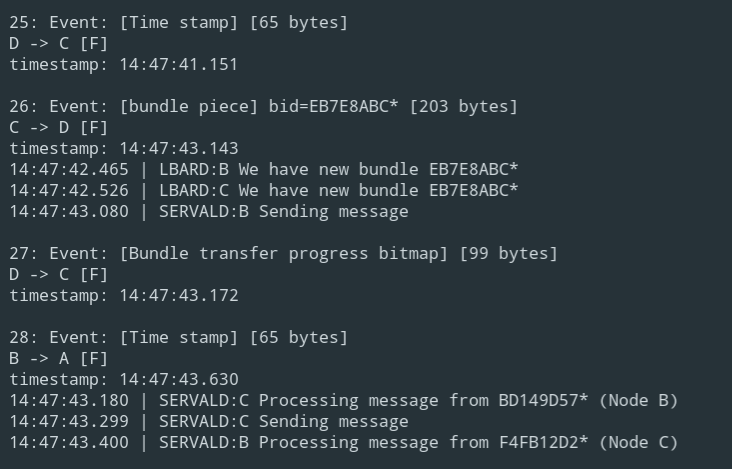
\includegraphics[width=15cm,height=15cm,keepaspectratio]{Figures/Chapter5-ASCIIRepresentation.png}
        \caption{ASCII Representation of test network}
        \label{fig:chapter5ASCIIRep}
    \end{centering}
\end{figure}
\todo{Make this into text instead of an image}

This output can then be piped to a file for debugging if testers do not have the requirements installed for generating the diagrams as outlined in the next sections.




\subsection{Generating a network diagram}
\todo{Change this to work in new structure} 
In the test definitions, it is often difficult to understand what the network topology of a given test is.
This is due to the fact that the topology definitions — while easy to understand for a computer — are not particularly friendly for humans to understand, due to their relatively complicated definition.
The topology definition are split into two sections, WiFi and Fakeradio, and lists connections only between two nodes — not the entire network.
\todo{Add more / fix this}
To render these diagrams, the layout will need to be extracted from the test definition, then a diagram drawn of this topology.
From this layout, the image will then need to be created and rendered.
There are two main solutions for creating the image: do it using a graphics library, or creating a DOT file and rendering it with Graphviz.
Using a graphics library would provide a high level of control over the creation of the image as graphical elements would need to be defined explicitly and as such are unlikely to have unforeseen side effects as could be expected with using a higher-level solution such as Graphviz.
That said, this would be considerably more complicated and harder to maintain than simply writing DOT files, then using the high-level tools provided by Graphviz to render this DOT file.
DOT files are text files that follow a specified syntax, and are used by Graphviz to render and create graphs.
These files are simple, and both human and machine-readable. 
After weighing these options it was decided that despite the far higher level of control possible by using a low-level graphics library, the accessibility, simplicity and maintainability of creating and rendering DOT files far outweighs this advantage.

To create the DOT files, minor modifications are needed to be made to the previously implemented line filtering as outlined in section \ref{filteringLines}.
The modifications are simple: when a WiFi or Fakeradio setup line is encountered the node information is stripped from these lines and saved to arrays.
How this is done depends on if it is a WiFi or a Fakeradio line.
For a Fakeradio line the program simply extracts the node numbers \todo{Show example?} from the line, converts these to the appropriate node character, and saves these two variables to a simple struct of just the two node characters.
This struct is appended to an array containing all the Fakeradio connections.
For a WiFi connection however this is slightly more complicated.
To determine the WiFi topology a 2D array is created.
When a line is encountered that lists a node being connected to a WiFi interface, the node character is appended to the array at the index of the interface.
An example of this data structure and the resultant network topology in \figurename{ \ref{fig:chapter5ResultWifiTopology}}.

\begin{figure}
    \begin{centering}
        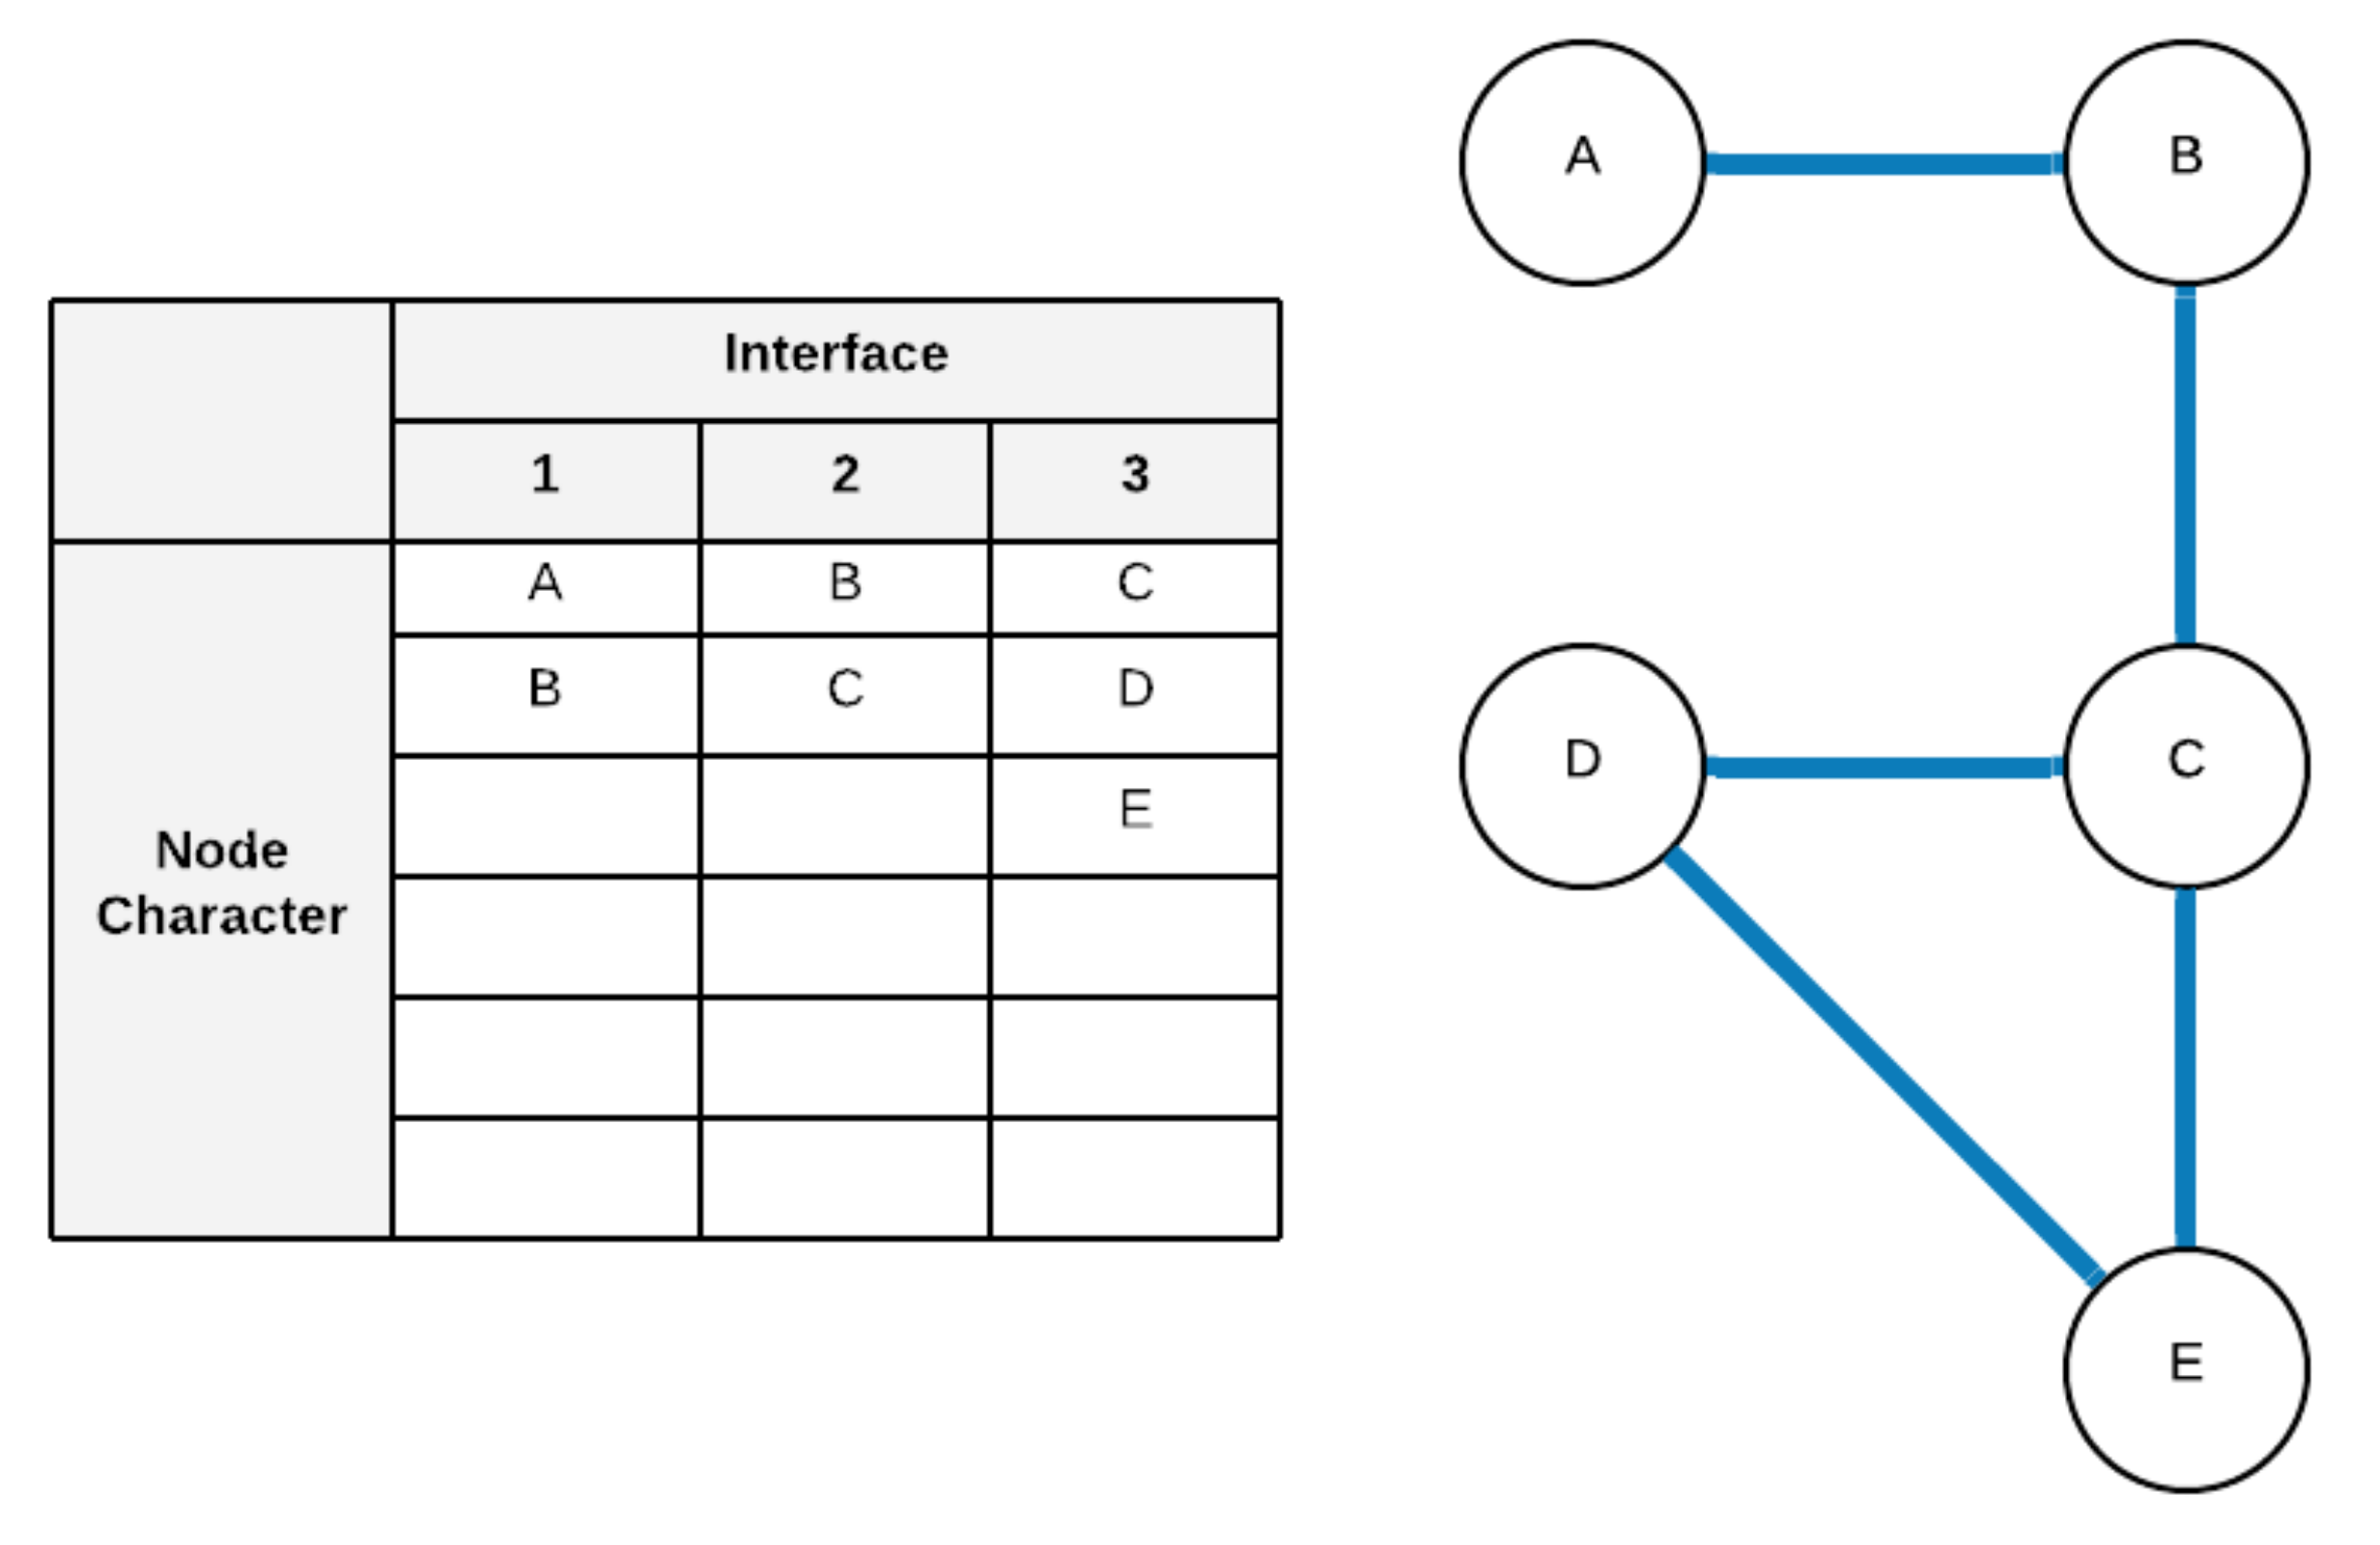
\includegraphics[width=15cm,height=10cm,keepaspectratio]{Figures/Chapter5-WifiArrayResult.png}
        \caption{WiFi Array and resultant topology}
        \label{fig:chapter5ResultWifiTopology}
    \end{centering}
\end{figure}

Once the simple log has finished being generated and the links between nodes gathered, the program then moves onto writing the layout DOT file.
The DOT file follows a simple format; initialisation of graph variables, and then the definition of the Layout sub-graph.
The graph is defined as a \emph{directed} graph.
While this may not appear to make sense initially — network traffic is not restricted by the direction — this is done for future-proofing: when this program will show network traffic, that \emph{will} be (partially) directed, and so this sub-graph is directed, however the direction hidden with the \verb|dir=none| flag.
Producing the DOT file consists of four steps:
\begin{enumerate}
    \item Open the file and write the initialisation
    \item Write the Fakeradio links
    \item Write the WiFi nodes
    \item Write the end of the DOT file, then close it
\end{enumerate}

In the first step, the program opens a new file with the name \verb|diagramLayout.dot|, and writes the initialisation variables.
This is simply writing a string listing all the graph variables. 
In \figurename{ \ref{fig:chapter5DotAndRender}} this would be from \verb|digraph A| to \verb|edge [dir=none, penwidth=3]|.

In the next step, the program simply iterates through all the Fakeradio links that have been saved, as outlined previously in this section.
Then this information is written to the DOT file with the extra field \verb|[color=red]|.
This is used to highlight Fakeradio links between nodes and help distinguish the different link types between nodes in a network.

Then, the program iterates through the WiFi link array. 
To do this, the program iterates through each of the interface arrays, and for each, simply creates all \emph{unique} combinations of the nodes in this interface.
With these combinations, the program then writes each unique combination to the file with the extra field \verb|[color=blue]|.

Finally, the program adds the closing curly braces to the file, and closes it.
The program then renders the DOT file with the command:

\verb|neato -Tpng [fileName] -o [outputFileName]|

\todo{Add a little of an outro/ summary}

\begin{figure}
    \begin{centering}
        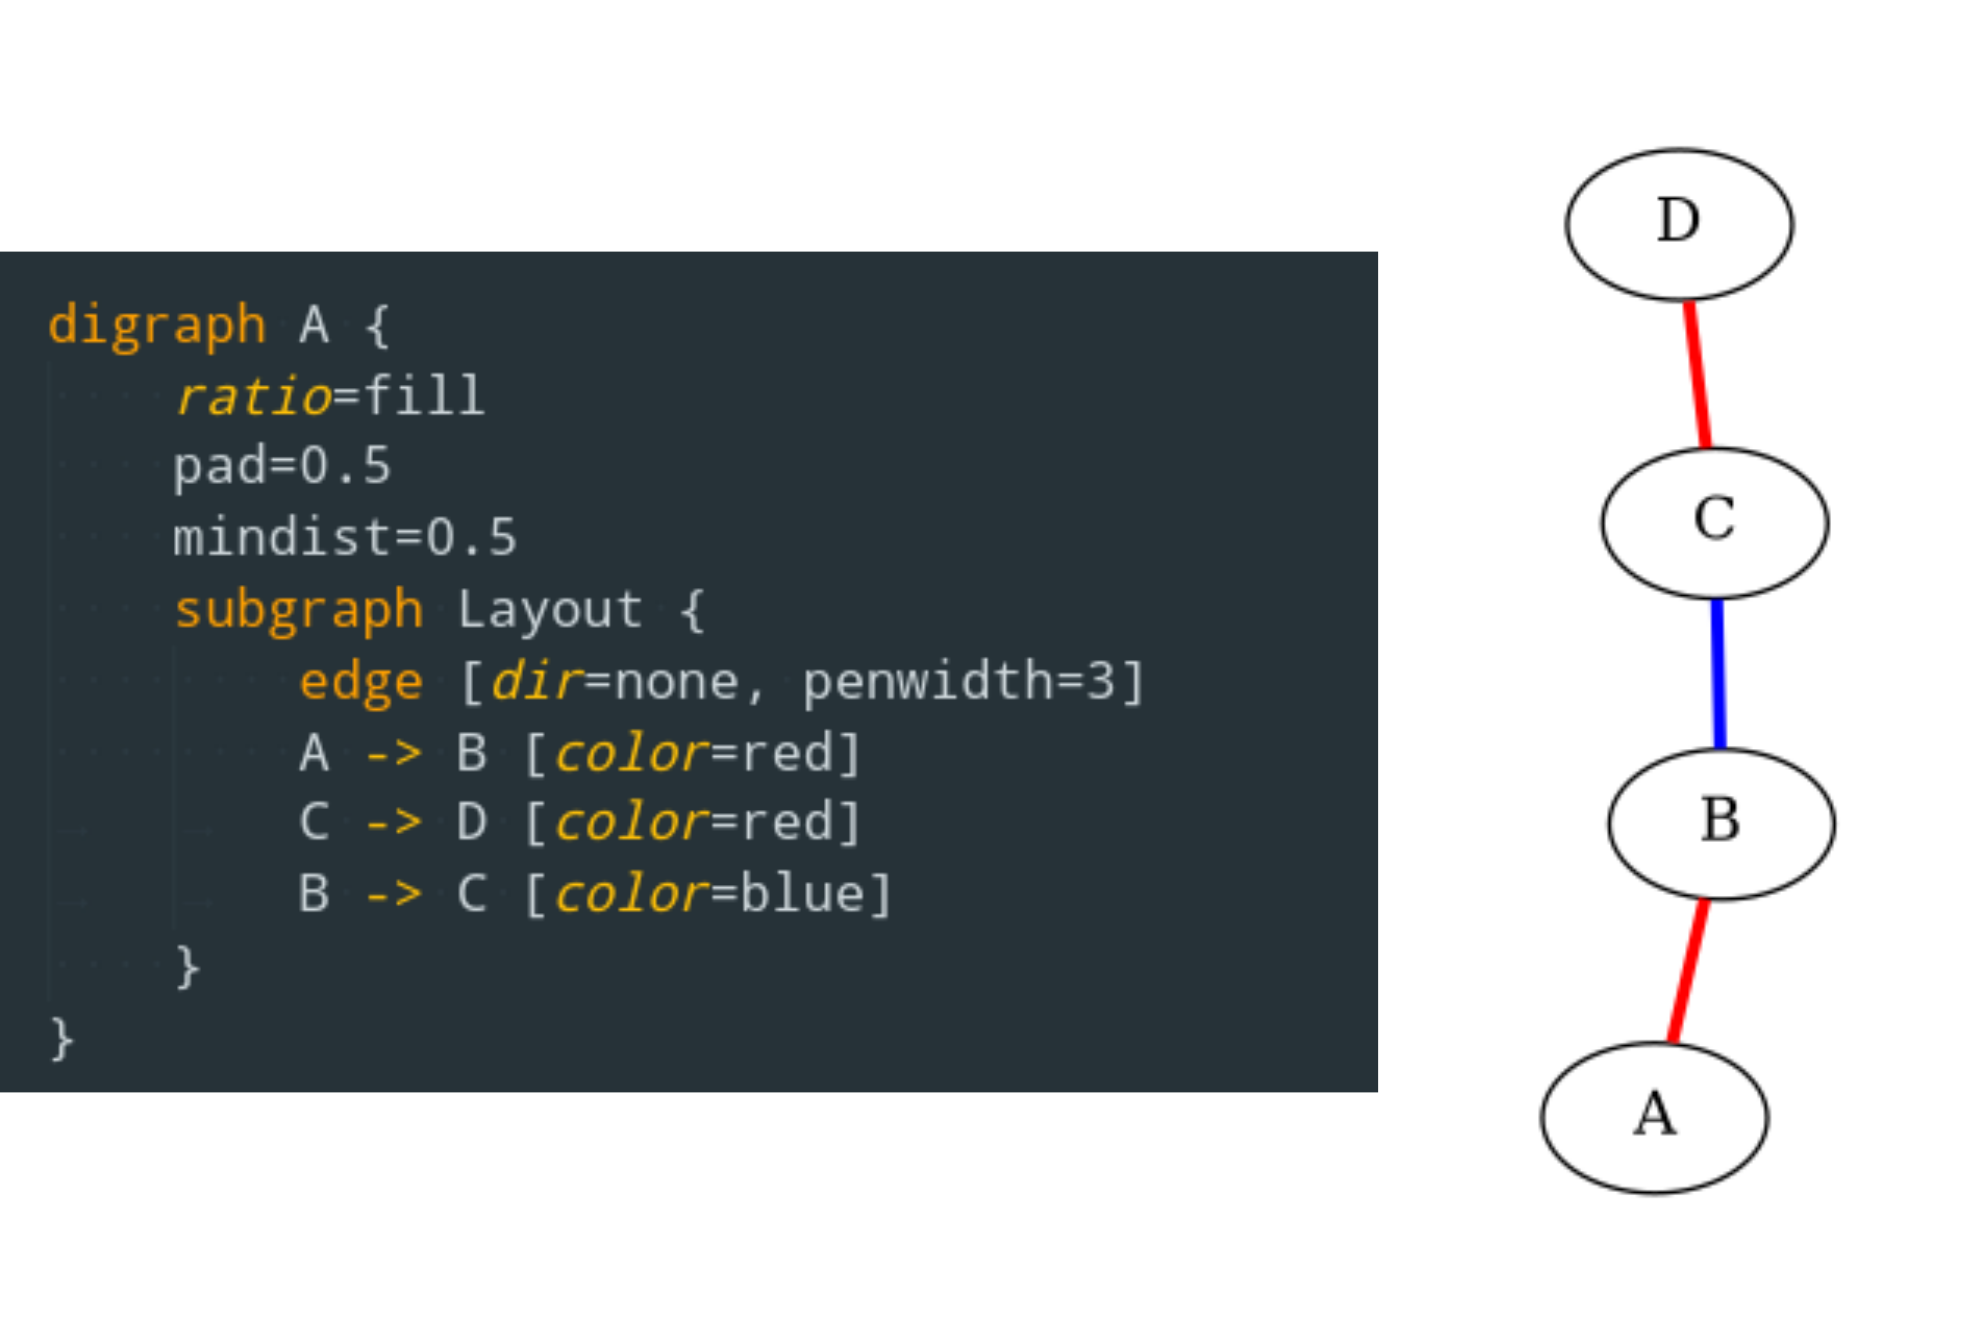
\includegraphics[width=15cm,height=10cm,keepaspectratio]{Figures/Chapter5-DotAndRender.png}
        \caption{Side-by-side of DOT file and output graph\\\emph{Rendered using neato}}
        \label{fig:chapter5DotAndRender}
    \end{centering}
\end{figure}


\subsection{Creating a LaTeX PDF}
\todo{Add intro}
\subsubsection{Transfer Diagrams}
The first step in creating a LaTeX PDF is to generate all the images of the network topology.
This is an extension of the development done in the previous section, however this is now creating multiple images — one per major event — and adding a directed link and label between a sending and receiving node.

To achieve this, the program iterates through every single major event in chronological order.
For each major event, the program adds the graph initialisation as previously outlined.
The program then adds a sub-graph named \emph{Transfer}.
The transfer sub-graph consists of just one line showing the \emph{directed} connection between the sending and receiving node.
To display the transfer in a nice format two options are added to this connection: the label, to show the transfer message, and the colour, which is the same as the normal colour of this link.


However, this had the issue that \verb|neato| will move the nodes around when a label is added that is longer than previously.
This is due to the fact that \verb|neato| will attempt to place all elements an even distance away from every element \emph{this includes labels}. 
To fix this issue, a sub-graph called \emph{Nodes} is created before the \emph{Transfer} sub-graph where it just lists all the nodes in the network, and applies the \verb|[pin=true]| flag to them.
This pins the nodes in their current position at the time the flag is added.
In this case, that is when \emph{just the nodes} have been placed.
This gives the program the ability to add labels of arbitrary length without moving the nodes around.
With this, the DOT files are all rendered, creating a chronologically ordered series of diagrams.

An example of a created DOT file can be seen in \figurename{ \ref{fig:chapter5DotAndRender}}.

\begin{figure}
    \begin{centering}
        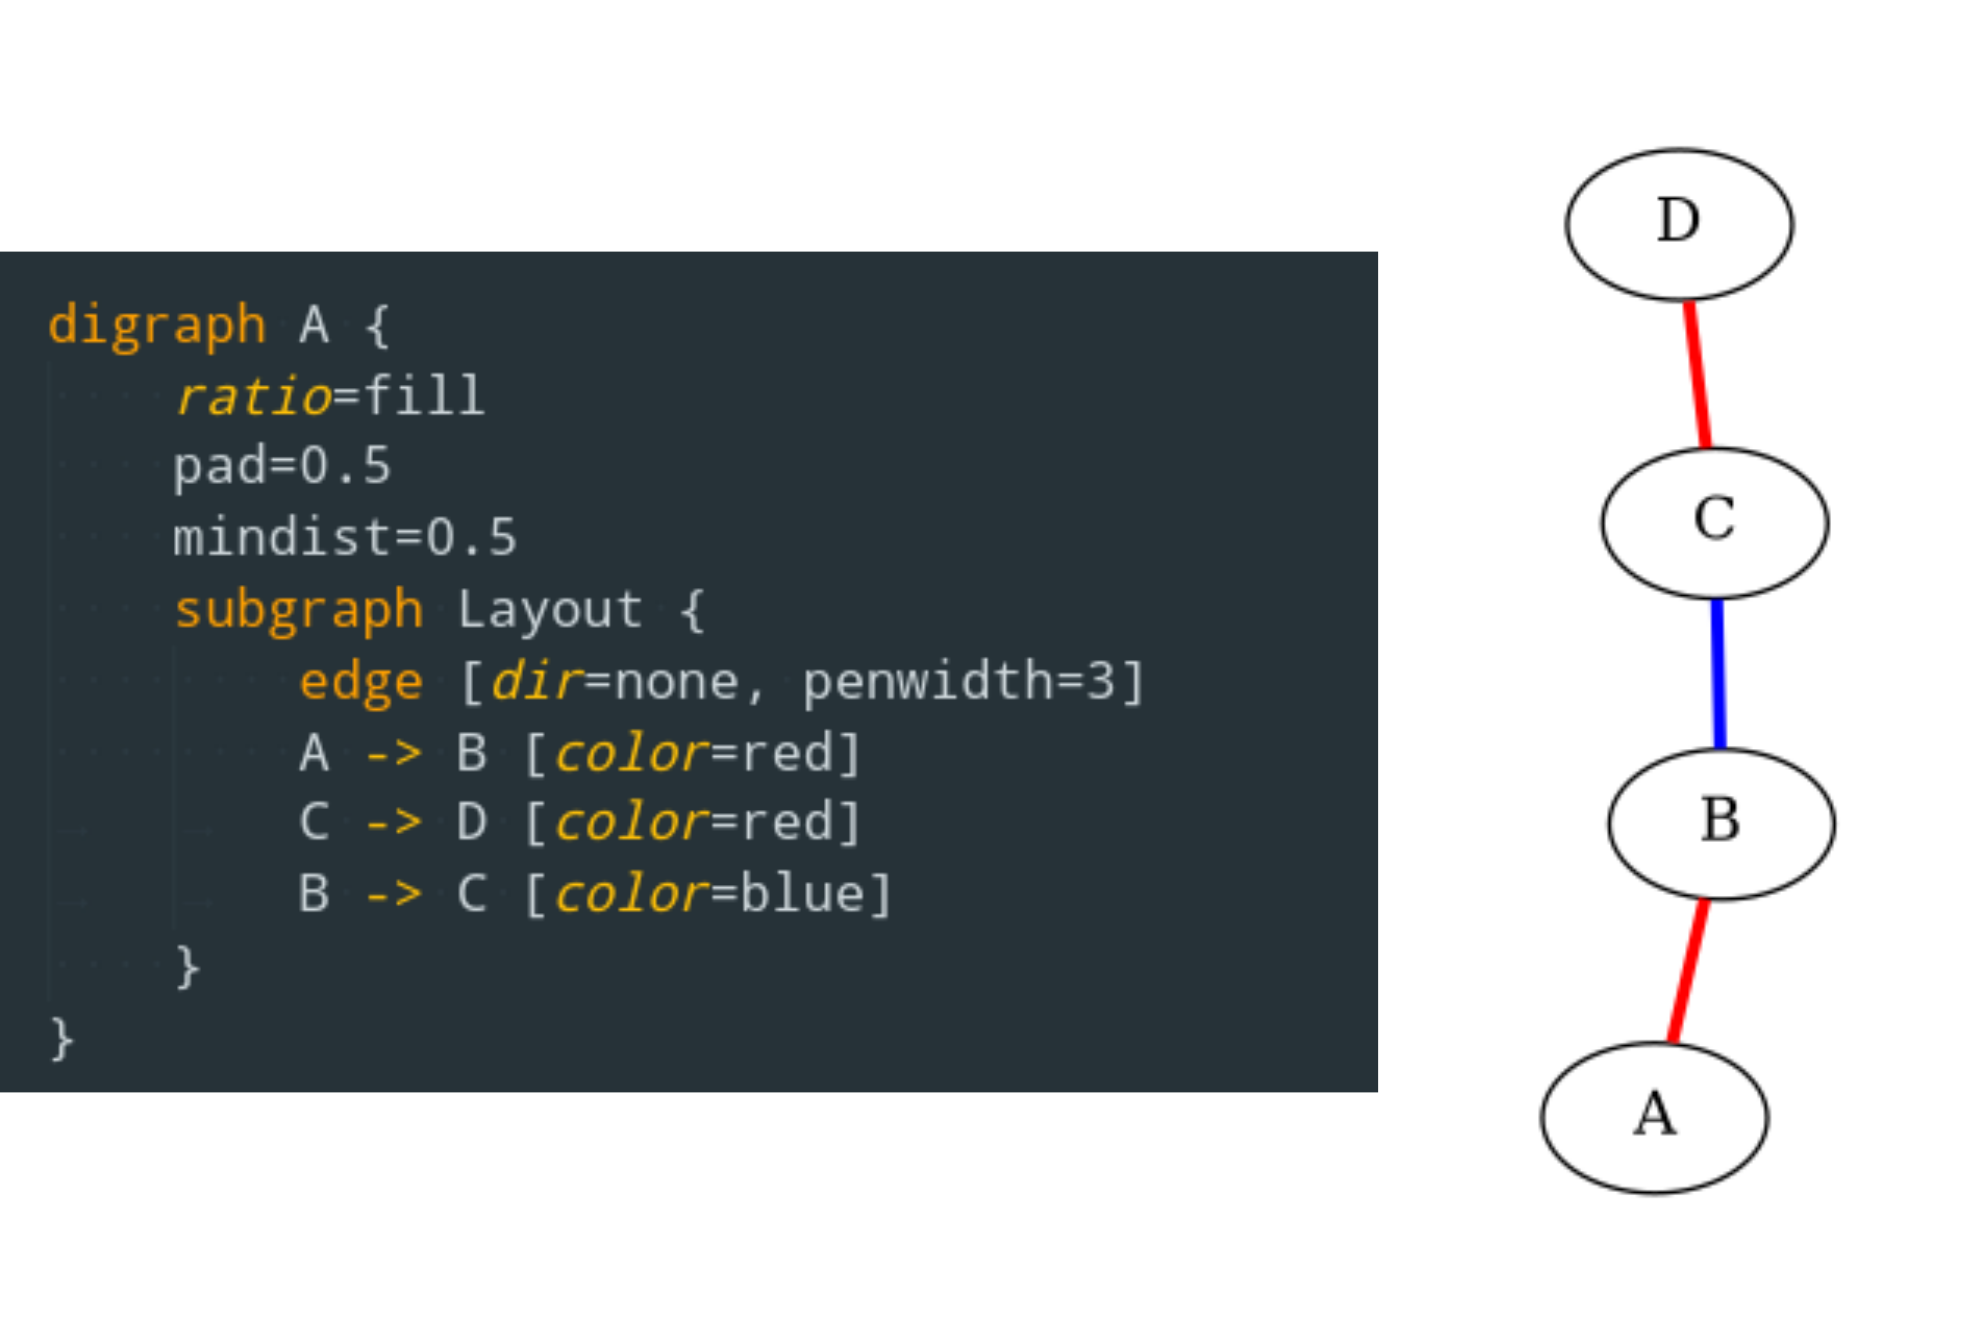
\includegraphics[width=15cm,height=10cm,keepaspectratio]{Figures/Chapter5-DotAndRender.png}
        \caption{Example of the major event DOT file side-by-side with the rendered diagram\\\emph{Rendered using neato}}
        \label{fig:chapter5TEMP}
    \end{centering}
\end{figure}
\todo{Change this to a different diagram}


However, one issue remains: while nodes themselves do not move around, the size of the page that a graph is drawn on \emph{will} change depending on the length of the label.
For the generation of just the images, there is not much that can be done to mitigate this. 
However, when the images are added to the LaTeX file as outlined in the next section, some mitigation can be done to reduce the amount of change between images on subsequent pages. 

\subsubsection{Creating the LaTeX PDF}
Once the diagrams have been created, a LaTeX PDF can then be created.
This PDF contains several pieces of information:
\begin{itemize}
    \item The test details
    \item A diagram for each major event
    \item All minor events associated with that major event
    \item The time the major event occurs
\end{itemize}
The produced LaTeX file follows a simple structure.
At the top of every page, the test details are listed. This is simply the name, result, and start/finish time of a test.
Underneath this, the time that the major event occurred is listed. 
The vast majority of the page is taken up by the diagram of the network layout, showing the network traffic when the major event occurs.
Finally, the bottom half of the page is a list of minor events associated with the major event.


To produce this, the program follows a simple process.
For the first major event, the program creates a new LaTeX file and writes the import and setup lines necessary for the compilation of the LaTeX document.
Then, the program simply writes the test det5ails to the file with the \verb|\large| tag.
The program then adds the image for that major event. Importantly, this image is \emph{right-aligned}. 
This is due to the fact that diagrams should roughly align with each-other throughout the document.
However, as mentioned previously, the page size will change depending on the length of the label.
As most diagrams should be produced with the topology on the right and the label on the left, this means that for the vast majority of the diagrams, the topology generated will all align on the right — however the distance between the topology and the left edge of the diagram may change.
By aligning the image along the right of the page, this should mean that — for the vast majority of cases — the variable width along the left of the diagram doesn't move the image.
After this, the program simply iterates through every minor event associated with the major event, and adds these lines to the LaTeX file.
Finally, a page break is added so that the next major event is put on a new page.
This is done for every major event.

Once the LaTeX file has been produced, the program renders the file using the command
\verb|pdflatex --output-directory=[output file] [file]|

\todo{Add image of pdf}

\section{Summary}

In this chapter we have continued answering the fourth research question: "How might these additional diagnostic tools be created and evaluated?" as started in Chapter 4.
These additional diagnostic tools were in the form of a C program that could be used to generate simpler, formatted, and chronologically ordered log files from the log files produced by the test framework, and optionally generate several different outputs displaying the network traffic throughout the test.

In \todo{reference section 1} the simple log generation was developed, and an explanation behind several design decisions were outlined.
In this section, the methodology and criteria of filtering lines was outlined, and the reasoning behind why these specific types of log lines were added to the simple log was listed.
Further, the output format of the simple log was listed, and the reasoning behind this format explained.

After this, the process for drawing the packet transfer throughout the network was detailed.
In this section the process was divided into four parts.
The first of these parts was categorising the log lines into major or minor events, where major events constituted a transfer of data between two nodes, and a minor event was any other useful information that would be displayed on the generated diagrams but was not a transfer.
The next part was developing an ASCII network diagram to be used by testers if they were lacking the required software (GraphViz and LaTeX) to generate the PDF.
In the third part, the method for generating network diagrams using DOT files was outlined, and the justifications for choosing GraphViz and DOT files were outlined.
Finally, these were combined to create the LaTeX document that is rendered into a PDF by the program. 
This PDF file contains a diagram of the network layout on every page for each major event, with a visual representation of the network traffic throughout the network at the time of this major event.
Under this diagram each of the minor events that are associated with this major event is listed in the same format as that of the simple log file.


In this chapter the outputs of the test framework were improved based on the improvements outlined in chapter 3.
Further, in this and the previous chapter, of the five improvements that were planned to be made to the LBARD test framework, four of them have now been implemented, with only the final one — "Validate the test framework against a real-world model of the network" — left to complete.
In the next chapter, the basis for validating the test framework against the real world will be implemented, and 
\todo{update after writing chapter 6}
